% +------------------------------------------------------------------------+
% | CGAL Reference Manual:  generators.tex
% +------------------------------------------------------------------------+
% | Geometric object generators.
% |
% | 09.06.1997   Lutz Kettner
% | 
\RCSdef{\generatorsRev}{$Revision$}
\RCSdefDate{\generatorsDate}{$Date$}
% +------------------------------------------------------------------------+

\ccParDims

\chapter{Geometric Object Generators}
\label{chapterGenerators}
\ccChapterRelease{\generatorsRev. \ \generatorsDate}\\
\ccChapterAuthor{Susan Hert}\\
\ccChapterAuthor{Michael Hoffmann}\\
\ccChapterAuthor{Lutz Kettner}

A variety of generators for geometric objects are provided in \cgal.
They are useful as synthetic test data sets, e.g.~for testing
algorithms on degenerate object sets and for performance analysis.

Section~\ref{sec:random_numbers_generator} describes a class for generating
random numbers.  Section~\ref{sec:generator_support} provides useful 
generic functions related to random
numbers like \ccc{random_selection()}. Section~\ref{sec:point_generators_2}
documents generators for two-dimensional point sets and Section~\ref{sec:point_generators_3} for three-dimensional point sets. 
Section~\ref{sec:segment_example} presents examples
using functions from Section~\ref{sectionGenericFunctions} to generate
composed objects, such as segments.  The generation of random convex sets
is described in Section~\ref{sec:building_random_convex_sets} and
Section~\ref{sec:random_simple_polygons} presents a function for 
generating random simple polygson.  Note that the \stl\ algorithm
\ccc{std::random_shuffle} is useful in this context to achieve random
permutations for otherwise regular generators (e.g.~points on a grid
or segment).

% +------------------------------------------------------------------------+

% =============================================================================
% The CGAL Reference Manual
% Chapter: Geometric Object Generators
% Section: Random Numbers Generator
% -----------------------------------------------------------------------------
% file  : doc_tex/support/Generator/Random.tex
% author: Sven Sch�nherr <sven@inf.ethz.ch>
% -----------------------------------------------------------------------------
% $CGAL_Chapter: Geometric Object Generators $
% $CGAL_Package: Random_numbers WIP $
% $Id$
% $Date$
% =============================================================================

\begin{ccRefClass}{Random}
\label{sec:random_numbers_generator}

% -----------------------------------------------------------------------------
\ccDefinition

The class \ccRefName is a random numbers generator. It generates
uniformly distributed random \ccc{bool}s, \ccc{int}s and \ccc{double}s. 
It can be used as the random number generating function object in the 
\stl\ algorithm \ccc{random_shuffle}.

Instances of \ccClassName\ can be seen as input streams. Different
streams are \emph{independent} of each other, i.e.\ the sequence of
numbers from one stream does \emph{not} depend upon how many numbers
were extracted from the other streams. At each time, an instance has 
a \emph{state} that uniquely determines the subsequent numbers being
produced.

It can be very useful, e.g.\ for debugging, to reproduce a sequence of
random numbers. This can be done by either initialising with a fixed
seed, or by using the state functions as described below.

\ccInclude{CGAL/Random.h}

% -----------------------------------------------------------------------------
\ccTypes

\ccUnchecked
\ccNestedType{State}{The State type.}

% -----------------------------------------------------------------------------
\ccCreation
\ccCreationVariable{random}

\ccConstructor{ Random( );}{
        introduces a variable \ccVar\ of type \ccClassTemplateName. The
        seed is chosen ``randomly'', depending on the system time.}

\ccConstructor{ Random( unsigned int seed);}{
        introduces a variable \ccVar\ of type \ccClassTemplateName\
        and initializes its internal state using \ccc{seed}. Equal
        values for \ccc{seed} result in equal sequences of random
        numbers.}

% -----------------------------------------------------------------------------
\ccOperations

\ccMemberFunction{ bool get_bool( );}{
        returns a random \ccc{bool}.}

\ccMemberFunction{ template <int b> int get_bits();}{
        returns a random \ccc{int} value from the interval
        $[\mbox{\ccc{0},\ccc{2^b}})$.  This is supposed to
	be efficient.}

\ccMemberFunction{ int get_int( int lower, int upper);}{
        returns a random \ccc{int} from the interval
        $[\mbox{\ccc{lower},\ccc{upper}})$. }

\ccMemberFunction{ double get_double( double lower = 0.0,
                                      double upper = 1.0);}{
        returns a random \ccc{double} from the interval
        $[\mbox{\ccc{lower},\ccc{upper}})$.}


\ccHeading{Distributions}

The following member functions are a 1-to-1 correspondence to
some distributions from the boost random library.


\ccMemberFunction{ template <typename IntType> IntType uniform_smallint( IntType lower=0, IntType upper=9);}{
        returns a random \ccc{IntType} from the interval
        $[\mbox{\ccc{lower},\ccc{upper}}]$. \ccc{IntType} can be an integral type 
        as \ccc{int}, \ccc{std::ptrdiff_t}, \ccc{std::size_t},etc. {\bf Warning: In contrast to \ccc{get_int} this function may return \ccc{upper}. }  }

\ccMemberFunction{ template <typename IntType> IntType uniform_int( IntType lower=0, IntType upper=9);}{
        returns a random \ccc{IntType} from the interval
        $[\mbox{\ccc{lower},\ccc{upper}}]$. \ccc{IntType} can be an integral type 
        as \ccc{int}, \ccc{std::ptrdiff_t}, \ccc{std::size_t},etc.  {\bf Warning: In contrast to \ccc{get_int} this function may return \ccc{upper}. } }

\ccMemberFunction{ template <typename RealType> Realtype uniform_real( RealType lower = 0.0,
                                      RealType upper = 1.0);}{
        returns a random \ccc{RealType} from the interval
        $[\mbox{\ccc{lower},\ccc{upper}})$. \ccc{RealType} can be \ccc{float}, \ccc{double}, etc.}

\ccMemberFunction{ template <typename RealType> RealType uniform_01();}{
        returns a random \ccc{RealType} from the interval
        $[0,1)$. \ccc{RealType} can be \ccc{float}, \ccc{double}, etc.}



\ccMemberFunction{ template <typename IntType> IntType operator() ( IntType upper);}{
        returns \ccVar\ccc{uniform_int<IntType>( 0, upper-1)}.}

% -----------------------------------------------------------------------------
\ccHeading{Seed and State Functions}

\ccMemberFunction{ unsigned int get_seed() const;}{
        returns the seed used for initialization.}

\ccMemberFunction{ void save_state( State& state) const;}{
        saves the current internal state in \ccc{state}.}

\ccMemberFunction{ void restore_state( State const& state);}{
        restores the internal state from \ccc{state}.}

% -----------------------------------------------------------------------------
\ccHeading{Equality Test}

\ccMemberFunction{ bool  operator == ( Random const& random2) const;}{
        returns \ccc{true}, iff \ccVar\ and \ccc{random2} have equal
        internal states.}

% -----------------------------------------------------------------------------
\ccImplementation

We use the boost random library function \ccc{boost::rand48} to generate the random
numbers.



\ccSeeAlso

\ccRefIdfierPage{CGAL::default_random}\\

\end{ccRefClass}

% ===== EOF ===================================================================


%\newpage
\section{Support Functions for Generators}
\label{sec:generator_support}
\ccThree{OutputIterator}{rand}{}


\subsection{{\it random\_selection()}}
\label{sec:random_selection}

\ccc{random_selection} chooses $n$ items at random from a random
access iterator range which is useful to produce degenerate input data
sets with multiple entries of identical items.

\ccInclude{CGAL/random_selection.h}

\ccFunction{template <class RandomAccessIterator, class Size, 
                      class OutputIterator, class Random>
    OutputIterator random_selection( RandomAccessIterator first,
        RandomAccessIterator last, 
        Size n, OutputIterator result, Random& rnd = default_random);}
{ chooses a random item from the range $[\ccc{first},\ccc{last})$ and
    writes it to \ccc{result}, each item from the range with equal
    probability, and repeats this $n$ times, thus writing $n$ items to
    \ccc{result}.
    A single random number is needed from \ccc{rnd} for each item.
    Returns the value of \ccc{result} after inserting the $n$ items.
    \ccPrecond \ccc{Random} is a random number generator type as provided 
    by the STL or by \ccc{Random}.
}


% +------------------------------------------------------------------------+
\section{2D Point Generators}
\label{sec:point_generators_2}
\lcTex{\ccIndexSubitemBegin[c]{generator}{2D point}}
\lcTex{\ccIndexSubitemBegin[c]{point, 2D}{generator}}

Two kinds of point generators are provided: first, random point
generators and second deterministic point generators. Most random
point generators and a few deterministic point generators are provided
as input iterators.  The input iterators model an infinite sequence of
points. The function \ccc{copy_n()} can be used to copy a
finite sequence; see Section~\ref{sectionCopyN}. The iterator adaptor
\ccc{Counting_iterator} can be used to create finite iterator
ranges; see Section~\ref{sectionCountingIterator}.
Other generators are provided as functions that write to output
iterators. Further functions add degeneracies or random perturbations.


% +------------------------------------------------------------------------+
\subsection{Point Generators as Input Iterators}
\lcTex{\ccIndexSubsubitemBegin[c]{generator}{2D point}{as input iterator}}

\ccDefinition

Input iterators are provided for random points uniformly distributed
over a two-dimensional domain (square or disc) or a one-dimensional
domain (boundary of a square, circle, or segment). Another input
iterator generates equally spaced points from a segment.

All iterators are parameterized with the point type \ccc{P} and all
with the exception of the class \ccc{Points_on_segment_2} have a second
template argument \ccc{Creator}, which defaults to the class
\ccc{Creator_uniform_2<double,P>}\footnote{%
  For compilers not supporting these kinds of default arguments, both
  template arguments must be provided when using these generators.}.
The \ccc{Creator} must be a function object accepting two \ccc{double}
values $x$ and $y$ and returning an initialized point \ccc{(x,y)} of type
\ccc{P}. Predefined implementations for these creators like the
default can be found in Section~\ref{sectionCreatorFunctionObjects}.
They simply assume an appropriate constructor for type \ccc{P}.

All generators know a range within which the coordinates of the
generated points will lie.

\ccInclude{CGAL/point_generators_2.h}

\ccTypes

The generators comply with the requirements of input iterators, which
include local type declarations including \ccc{value_type}, 
denoted by \ccc{P} here.

\ccCreation
\ccTwo{}{\hspace*{11cm}}
%% \ccTwo{}{\hspace*{10cm}}

\ccHtmlNoClassFile
\begin{ccClassTemplate}{Random_points_in_disc_2<P,Creator>}
\ccCreationVariable{g}
\ccConstructor{Random_points_in_disc_2( double r, Random& rnd =
  default_random);}{%
  $g$ is an input iterator creating points of type \ccc{P} uniformly
  distributed in the open disc with radius $r$,
  i.e.~$|\ccc{*g}| < r$~. Two random numbers are needed from
  \ccc{rnd} for each point.
} 
\end{ccClassTemplate}

\ccHtmlNoClassFile
\begin{ccClassTemplate}{Random_points_on_circle_2<P,Creator>}
\ccCreationVariable{g}
\ccConstructor{Random_points_on_circle_2( double r, Random& rnd =
  default_random);}{%
  $g$ is an input iterator creating points of type \ccc{P} uniformly
  distributed on the circle with radius $r$,
  i.e.~$|\ccc{*g}| == r$~. A single random number is needed from
  \ccc{rnd} for each point.
} 
\end{ccClassTemplate}

\ccHtmlNoClassFile
\begin{ccClassTemplate}{Random_points_in_square_2<P,Creator>}
\ccCreationVariable{g}
\ccConstructor{Random_points_in_square_2( double a, Random& rnd =
  default_random);}{%
  $g$ is an input iterator creating points of type \ccc{P} uniformly
  distributed in the half-open square with side length $2 a$, centered
  at the origin, i.e.~$\forall p = \ccc{*g}:  -a \le p.x() < a$ and 
  $-a \le p.y() < a$~. 
  Two random numbers are needed from \ccc{rnd} for each point.
} 
\end{ccClassTemplate}

\ccHtmlNoClassFile
\begin{ccClassTemplate}{Random_points_on_square_2<P,Creator>}
\ccCreationVariable{g}
\ccConstructor{Random_points_on_square_2( double a, Random& rnd =
  default_random);}{%
  $g$ is an input iterator creating points of type \ccc{P} uniformly
  distributed on the boundary of the square with side length $2 a$,
  centered at the origin, i.e.~$\forall p = \ccc{*g}:$ one
  coordinate is either $a$ or $-a$ and for the 
  other coordinate $c$ holds $-a \le c < a$~.
  A single random number is needed from \ccc{rnd} for each point.
} 
\end{ccClassTemplate}

\ccHtmlNoClassFile
\begin{ccClassTemplate}{Random_points_on_segment_2<P,Creator>}
\ccCreationVariable{g}
\ccConstructor{Random_points_on_segment_2( const P& p, const P& q,
  Random& rnd = default_random);}{%
  $g$ is an input iterator creating points of type \ccc{P} uniformly
  distributed on the segment from $p$ to $q$ (excluding $q$),
  i.e.~$\ccc{*g} == (1-\lambda)\, p + \lambda q$ where $0 \le \lambda < 1$~.
  A single random number is needed from \ccc{rnd} for each point.
  \ccPrecond The expressions \ccc{to_double(p.x())} and
    \ccc{to_double(p.y())} must  result in the respective
    \ccc{double} representation of the coordinates of $p$,
    and similarly for $q$.}

\end{ccClassTemplate}

\ccHtmlNoClassFile
\begin{ccClassTemplate}{Points_on_segment_2<P>}
\ccCreationVariable{g}
\ccConstructor{Points_on_segment_2( const P& p, const P& q, 
                                    std::size_t n, std::size_t i = 0);}{%
  $g$ is an input iterator creating points of type \ccc{P} equally 
  spaced on the segment from $p$ to $q$. $n-i$ points are placed on the
  segment defined by $p$ and $q$. Values of the index parameter $i$ larger 
  than 0 indicate starting points for the sequence further from $p$.
  Point $p$ has index value 0 and $q$ has index value $n-1$.
  \ccPrecond The expressions \ccc{to_double(p.x())} and
    \ccc{to_double(p.y())} must  result in the respective
    \ccc{double} representation of the coordinates of $p$, and similarly 
    for $q$.}


\ccOperations
\ccThree{double}{g.source();}{}
\lcTex{\ccAutoIndexingOff}
\ccMethod{double range();}{returns the range in which the point
  coordinates lie, i.e.~$\forall x: |x| \leq $\ccc{range()} and
  $\forall y: |y| \leq $\ccc{range()}.}%
\lcTex{\ccIndexSubitem[C]{range}{\ccFont Random_points_*_2}}

The generators \ccc{Random_points_on_segment_2} and
\ccc{Points_on_segment_2} have two additional methods.

\ccMethod{const P& source();}{returns the source point of the segment.}%
\lcTex{
\ccIndexSubitem[C]{source}{\ccFont Random_points_on_segment_2}%
\ccIndexSubitem[C]{source}{\ccFont Points_on_segment_2}%
}%
\ccGlue
\ccMethod{const P& target();}{returns the target point of the segment.}
\lcTex{
\ccIndexSubitem[C]{target}{\ccFont Random_points_on_segment_2}%
\ccIndexSubitem[C]{target}{\ccFont Points_on_segment_2}%
\ccAutoIndexingOn
}%

\end{ccClassTemplate}


\ccSeeAlso

\ccc{std::random_shuffle}, \ccc{random_selection}, 
\ccc{copy_n}, \ccc{Counting_iterator},
\ccTexHtml{\\}{}
\ccc{Join_input_iterator_1}.
\lcTex{\ccIndexSubsubitemEnd[c]{generator}{2D point}{as input iterator}}


% +------------------------------------------------------------------------+
\subsection{Point Generators as Functions}
\lcTex{\ccIndexSubsubitemBegin[c]{generator}{2D point}{as function}}

\ccHeading{Grid Points}
\ccThree{OutputIterator}{rand}{}
\lcTex{\ccIndexSubsubitem[c]{generator}{2D point}{on grid}}

Grid points are generated by functions that write to output iterators.

\def\ccLongParamLayout{\ccTrue}
\ccFunction{template <class OutputIterator, Creator creator>
    OutputIterator
    points_on_square_grid_2( double a, std::size_t n, OutputIterator o,
                             Creator creator = 
                             Creator_uniform_2<double,P>);}
{ creates the first $n$ points on the regular $\lceil\sqrt{n}\,\rceil
    \times \lceil  \sqrt{n}\,\rceil$ grid within the square
    $[-a,a]\times [-a,a]$. Returns the value of $o$ after inserting
    the $n$ points. 
    \ccPrecond \ccc{Creator} must be a function object accepting two
    \ccc{double} values $x$ and $y$ and returning an initialized point
    \ccc{(x,y)} of type \ccc{P}. Predefined implementations for these
    creators like the default can be found in
    Section~\ref{sectionCreatorFunctionObjects}. The
    \ccc{OutputIterator} must accept values of type \ccc{P}. If the
    \ccc{OutputIterator} has a \ccc{value_type} the default
    initializer of the \ccc{creator} can be used. \ccc{P} is set to
    the \ccc{value_type} in this case.}
\def\ccLongParamLayout{\ccFalse}


\ccFunction{template <class P, class OutputIterator>
    OutputIterator points_on_segment_2( const P& p, const P& q, std::size_t n,
    OutputIterator o);}
{ creates $n$ points equally spaced on the segment from $p$ to $q$,
    i.e.~$\forall i: 0 \le i < n: o[i] := \frac{n-i-1}{n-1}\, p +
    \frac{i}{n-1}\, q$. Returns the value of $o$ after inserting
    the $n$ points.}

\ccHeading{Random Perturbations}
\ccIndexMainItem{random perturbations}

Degenerate input sets like grid points can be randomly perturbed by a
small amount to produce {\em quasi}-degenerate test sets. This
challenges numerical stability of algorithms using inexact arithmetic and
exact predicates to compute the sign of expressions slightly off from zero.

\ccFunction{template <class ForwardIterator>
    void perturb_points_2( ForwardIterator first, ForwardIterator last, 
        double xeps, double yeps = xeps, Random& rnd = default_random,
        Creator creator = Creator_uniform_2<double,P>);}
{ perturbs the points in the range $[\ccc{first},\ccc{last})$ by
  replacing each point with a random point from the 
  \ccc{xeps} $\times$ \ccc{yeps} rectangle centered at the original point.
  Two random numbers are needed from \ccc{rnd} for each point.
  \ccPrecond   \ccc{Creator} must be a function object accepting two
    \ccc{double} values $x$ and $y$ and returning an initialized point
    \ccc{(x,y)} of type \ccc{P}. Predefined implementations for these
    creators like the default can be found in
    Section~\ref{sectionCreatorFunctionObjects}. The \ccc{value_type} of the
    \ccc{ForwardIterator} must be assignable to \ccc{P}.
    \ccc{P} is equal to the \ccc{value_type} of the
    \ccc{ForwardIterator} when using the default initializer.
    The expressions \ccc{to_double((*first).x())} and
    \ccc{to_double((*first).y())} must result in the respective
    coordinate values.
}

\ccHeading{Adding Degeneracies}
\ccModifierCrossRefOff
\ccIndexSubitem{degeneracies}{adding to input}
\ccModifierCrossRefOn

For a given point set certain kinds of degeneracies can be produced
adding new points. The \ccc{random_selection()} function is
useful for generating multiple copies of identical points; see
Section~\ref{sec:random_selection}. The
\ccc{random_collinear_points_2()} function adds collinearities to
a point set.


\def\ccLongParamLayout{\ccTrue}
\ccFunction{template <class RandomAccessIterator, class OutputIterator>
    OutputIterator random_collinear_points_2( RandomAccessIterator first,
        RandomAccessIterator last, 
        std::size_t n, OutputIterator first2, Random& rnd = default_random,
        Creator creator = Creator_uniform_2<double,P>);}
{ randomly chooses two points from the range $[\ccc{first},\ccc{last})$,
    creates a random third point on the segment connecting these two
    points, writes it to \ccc{first2}, and repeats this $n$ times, thus
    writing $n$ points to \ccc{first2} that are collinear with points
    in the range $[\ccc{first},\ccc{last})$.
    Three random numbers are needed from \ccc{rnd} for each point.
    Returns the value of \ccc{first2} after inserting the $n$ points.
  \ccPrecond  \ccc{Creator} must be a function object accepting two
    \ccc{double} values $x$ and $y$ and returning an initialized point
    \ccc{(x,y)} of type \ccc{P}. Predefined implementations for these
    creators like the default can be found in
    Section~\ref{sectionCreatorFunctionObjects}. The \ccc{value_type} of the
    \ccc{RandomAccessIterator} must be assignable to \ccc{P}.
    \ccc{P} is equal to the \ccc{value_type} of the
    \ccc{RandomAccessIterator} when using the default initializer.
    The expressions \ccc{to_double((*first).x())} and
    \ccc{to_double((*first).y())} must result in the respective
    coordinate values.
}
\def\ccLongParamLayout{\ccFalse}
\lcTex{\ccIndexSubsubitemEnd[c]{generator}{2D point}{as function}}


\ccSeeAlso

\ccc{std::random_shuffle}, \ccc{random_selection}.

\ccExample

We want to generate a test set of 1000 points, where 60\% are chosen
randomly in a small disc, 20\% are from a larger grid, 10\% are duplicates
points, and 10\% collinear points. A random shuffle removes the
construction order from the test set. See \ccTexHtml{%
Figure~\ref{figurePointGenerator}}{Figure <A HREF="#PointGenerators">
  <IMG SRC="cc_ref_up_arrow.gif" ALT="reference arrow" WIDTH="10"
  HEIGHT="10"></A>} for the example output.

\ccIncludeExampleCode{Generator/generators_prog1.C}

\begin{ccTexOnly}
  \begin{figure}
    \noindent
    \hspace*{0.025\textwidth}%
    \begin{minipage}{0.45\textwidth}%
      \includegraphics[width=\textwidth]{generators_prog1.ps}
      \caption{Output of example program for point generators.}
      \label{figurePointGenerator}
    \end{minipage}%
    \hspace*{0.05\textwidth}%
    \begin{minipage}{0.45\textwidth}%
      \includegraphics[width=\textwidth]{generators_prog2.ps}
      \caption{Output of example program for point generators working
        on integer points.}
      \label{figureIntegerPointGenerator}
    \end{minipage}%
  \end{figure}
\end{ccTexOnly}

\begin{ccHtmlOnly}
  <A NAME="PointGenerators">
  <TABLE><TR><TD ALIGN=LEFT VALIGN=TOP WIDTH=60%>
    <A HREF="./generators_prog1.gif">Figure:</A>
    Output of example program for point generators.
  </TD><TD ALIGN=LEFT VALIGN=TOP WIDTH=5% NOWRAP>
  </TD><TD ALIGN=LEFT VALIGN=TOP WIDTH=35% NOWRAP>
    <A HREF="./generators_prog1.gif">
        <img src="./generators_prog1_small.gif" 
             alt="Point Generator Example Output"></A>
  </TD></TR></TABLE>
\end{ccHtmlOnly}

%\newpage

The second example demonstrates the point generators with integer
points. Arithmetic with \ccc{double}s is sufficient to produce
regular integer grids. See \ccTexHtml{%
Figure~\ref{figureIntegerPointGenerator}}{Figure 
  <A HREF="#IntegerPointGenerators">
  <IMG SRC="cc_ref_up_arrow.gif" ALT="reference arrow" WIDTH="10"
  HEIGHT="10"></A>}
for the example output.

\ccIncludeExampleCode{Generator/generators_prog2.C}

\begin{ccHtmlOnly}
  <A NAME="IntegerPointGenerators">
  <TABLE><TR><TD ALIGN=LEFT VALIGN=TOP WIDTH=60%>
    <A HREF="./generators_prog2.gif">Figure:</A>
        Output of example program for point generators working
        on integer points.
  </TD><TD ALIGN=LEFT VALIGN=TOP WIDTH=5% NOWRAP>
  </TD><TD ALIGN=LEFT VALIGN=TOP WIDTH=35% NOWRAP>
    <A HREF="./generators_prog2.gif">
        <img src="./generators_prog2_small.gif" 
             alt="Integer Point Generator Example Output"></A>
  </TD></TR></TABLE>
\end{ccHtmlOnly}%
\lcTex{
\ccIndexSubitemEnd[c]{generator}{2D point}%
\ccIndexSubitemEnd[c]{point, 2D}{generator}%
}


% +------------------------------------------------------------------------+
\newpage
\section{3D Point Generators}
\label{sec:point_generators_3}
\lcTex{
\ccIndexSubitemBegin[c]{generator}{3D point}
\ccIndexSubitemBegin[c]{point, 3D}{generator}
}

One kind of point generator is currently provided for 3D points: Random point
generators implemented as input iterators.  The input iterators model
an infinite sequence of points. The function \ccc{copy_n()} can
be used to copy a finite sequence, see Section~\ref{sectionCopyN}. The
iterator adaptor \ccc{Counting_iterator} can be used to create
finite iterator ranges, see Section~\ref{sectionCountingIterator}.


% +------------------------------------------------------------------------+
\subsection{Point Generators as Input Iterators}

\ccDefinition

Input iterators are provided for random points uniformly distributed
in a three-dimensional volume (sphere or cube) or a two-dimensional
surface (boundary of a sphere).

All iterators are parameterized with the point type \ccc{P} and a second
template argument \ccc{Creator} which defaults to
\ccc{Creator_uniform_3<double,P>}\footnote{%
  For compilers not supporting these kinds of default arguments, both
  template arguments must be provided when using these generators.}.
The \ccc{Creator} must be a function object accepting three
\ccc{double} values $x$, $y$ and $z$ and returning an initialized
point \ccc{(x,y,z)} of type \ccc{P}. Predefined implementations for
these creators like the default can be found in
Section~\ref{sectionCreatorFunctionObjects}.  They simply assume an
appropriate constructor for type \ccc{P}.

All generators know a range within which the coordinates of the
generated points will lie.

\ccInclude{CGAL/point_generators_3.h}

\ccTypes

The generators comply with the requirements of input iterators, which
include local type declarations including \ccc{value_type}, denoted by 
\ccc{P} here.

\ccCreation
\ccTwo{}{\hspace*{11cm}}

\ccHtmlNoClassFile
\begin{ccClassTemplate}{Random_points_in_sphere_3<P,Creator>}
\ccCreationVariable{g}
\ccConstructor{Random_points_in_sphere_3( double r, Random& rnd =
  default_random);}{%
  $g$ is an input iterator creating points of type \ccc{P} uniformly
  distributed in the open sphere with radius $r$,
  i.e.~$|\ccc{*g}| < r$~.  Three random numbers are needed from
  \ccc{rnd} for each point.
} 
\end{ccClassTemplate}

\ccHtmlNoClassFile
\begin{ccClassTemplate}{Random_points_on_sphere_3<P,Creator>}
\ccCreationVariable{g}
\ccConstructor{Random_points_on_sphere_3( double r, Random& rnd =
  default_random);}{%
  $g$ is an input iterator creating points of type \ccc{P} uniformly
  distributed on the boundary of a sphere with radius $r$,
  i.e.~$|\ccc{*g}| == r$~. Two random numbers are needed from
  \ccc{rnd} for each point.
} 
\end{ccClassTemplate}

\ccHtmlNoClassFile
\begin{ccClassTemplate}{Random_points_in_cube_3<P,Creator>}
\ccCreationVariable{g}
\ccConstructor{Random_points_in_cube_3( double a, Random& rnd =
  default_random);}{%
  $g$ is an input iterator creating points of type \ccc{P} uniformly
  distributed in the half-open cube with side length $2 a$, centered
  at the origin, i.e.~$\forall p = \ccc{*g}:  -a \le p.x(),p.y(),p.z() < a$~. 
  Three random numbers are needed from \ccc{rnd} for each point.
} 
\end{ccClassTemplate}
\lcTex{
\ccIndexSubitemEnd[c]{generator}{3D point}
\ccIndexSubitemEnd[c]{point, 3D}{generator}
}


\ccSeeAlso

\ccc{std::random_shuffle}, \ccc{random_selection}, 
\ccc{copy_n}, \ccc{Counting_iterator}, 
\ccTexHtml{\\}{}
\ccc{Join_input_iterator_1}.


% +------------------------------------------------------------------------+
%\newpage
\section{Examples Generating Segments}
\label{sec:segment_example}
\lcTex{\ccIndexSubitemBegin[c]{generator}{segment}}

The following two examples illustrate the use of the generic functions
from Section~\ref{sectionGenericFunctions} like
\ccc{Join_input_iterator_2}%
\lcTex{\ccIndexGlobalFunction{Join_input_iterator_2}} to generate 
composed objects from other
generators -- here two-dimensional segments from two point generators.

We want to generate a test set of 200 segments, where one endpoint is
chosen randomly from a horizontal segment of length 200, and the other
endpoint is chosen randomly from a circle of radius 250. See
\ccTexHtml{Figure~\ref{figureSegmentGenerator}}{Figure <A
  HREF="#SegmentGenerator"> <IMG SRC="cc_ref_up_arrow.gif"
  ALT="reference arrow" WIDTH="10" HEIGHT="10"></A>} for the example
output.

\begin{ccTexOnly}
  \begin{figure}
    \noindent
    \hspace*{0.025\textwidth}%
    \begin{minipage}[t]{0.45\textwidth}%
      \includegraphics[width=\textwidth]{Segment_generator_prog1.ps}
      \caption{Output of the first example program for the generic generator.}
      \label{figureSegmentGenerator}
    \end{minipage}%
    \hspace*{0.05\textwidth}%
    \begin{minipage}[t]{0.45\textwidth}%
      \includegraphics[width=\textwidth]{Segment_generator_prog2.ps}
      \caption{Output of the second example program for the generic
        generator without using intermediate storage.}
      \label{figureSegmentGeneratorFan}
    \end{minipage}%
  \end{figure}
\end{ccTexOnly}

\ccIncludeExampleCode{Generator/Segment_generator_prog1.C}

\begin{ccHtmlOnly}
  <A NAME="SegmentGenerator">
  <TABLE><TR><TD ALIGN=LEFT VALIGN=TOP WIDTH=60%>
    <A HREF="./Segment_generator_prog1.gif">Figure:</A>
    Output of example program for the generic segment generator.
  </TD><TD ALIGN=LEFT VALIGN=TOP WIDTH=5% NOWRAP>
  </TD><TD ALIGN=LEFT VALIGN=TOP WIDTH=35% NOWRAP>
    <A HREF="./Segment_generator_prog1.gif">
        <img src="./Segment_generator_prog1_small.gif" 
             alt="Segment Generator Example Output"></A>
  </TD></TR></TABLE>
\end{ccHtmlOnly}

The second example generates a regular structure of 100 segments; see 
\ccTexHtml{Figure~\ref{figureSegmentGeneratorFan}}{Figure <A
  HREF="#SegmentGeneratorFan"> <IMG SRC="cc_ref_up_arrow.gif"
  ALT="reference arrow" WIDTH="10" HEIGHT="10"></A>} for the example
output. It uses the \ccc{Points_on_segment_2}%
\lcTex{\ccIndexGlobalFunction{Points_on_segment_2}} iterator,
\ccc{Join_input_iterator_2}%
\lcTex{\ccIndexGlobalFunction{Join_input_iterator_2}}
and \ccc{Counting_iterator}%\lcTex{\ccIndexGlobalFunction{Counting_iterator}}
to avoid any intermediate storage of the generated objects until they are
used, which in this example means copied to a window stream.

\ccIncludeExampleCode{Generator/Segment_generator_prog2.C}

\begin{ccHtmlOnly}
  <A NAME="SegmentGeneratorFan">
  <TABLE><TR><TD ALIGN=LEFT VALIGN=TOP WIDTH=60%>
    <A HREF="./Segment_generator_prog2.gif">Figure:</A>
    Output of example program for the generic segment generator using
    pre-computed point locations.
  </TD><TD ALIGN=LEFT VALIGN=TOP WIDTH=5% NOWRAP>
  </TD><TD ALIGN=LEFT VALIGN=TOP WIDTH=35% NOWRAP>
    <A HREF="./Segment_generator_prog2.gif">
        <img src="./Segment_generator_prog2_small.gif" 
             alt="Segment Generator Example Output 2"></A>
  </TD></TR></TABLE>
\end{ccHtmlOnly}
\lcTex{\ccIndexSubitemEnd[c]{generator}{segment}}


% +--------------------------------------------------------+
% restore default column and paragraph layout
\ccParDims
\cgalColumnLayout

%% ==============================================================
%% Specification: Random Convex Sets
%% --------------------------------------------------------------
%% file  : rcs_spec.awi
%% author: Michael Hoffmann
%% maintainer: Susan Hert 
%% $Id$
%% ==============================================================

\RCSdef{\RandomConvexSetRev}{$Revision$}
\RCSdefDate{\RandomConvexSetDate}{$Date$}

\newpage

\ccParDims

\section{Building Random Convex Sets}
\label{section_BuildingRandomConvexSets}
\lcTex{\ccIndexMainItem[c]{random convex set}}

This section describes a function to compute a random convex planar
point set of given size where the points are drawn from a specific
domain.

\ccInclude{CGAL/random_convex_set_2.h}

\def\ccLongParamLayout{\ccTrue} 

\ccGlobalFunction{template < class OutputIterator, class Point_generator,
  class Traits > OutputIterator random_convex_set_2( int n,
  OutputIterator o, const Point_generator& pg, Traits t =
  Default_traits);}

computes a random convex \ccc{n}-gon by writing its vertices (oriented
counterclockwise) to \ccc{o}. The resulting polygon is scaled such
that it fits into the bounding box as specified by \ccc{pg}. Therefore
we cannot easily describe the resulting distribution.

\ccHeading{Precondition}
\begin{enumerate}
\item \ccc{Point_generator} satisfies the requirements stated in
  section \ref{point_generator_req},
\item If \ccc{Traits} is specified, it has to satisfy the
  requirements stated in section \ref{req_random_convex_sets_traits}
  and \ccc{Traits::Point_2} must be the same as
  \ccc{Point_generator::value_type},
\item if \ccc{Traits} is not specified,
  \ccc{Point_generator::value_type} must be \ccc{Point_2<
    R >} for some representation class \ccc{R},
\item \ccc{OutputIterator} accepts
  \ccc{Point_generator::value_type} as value type {\it and}
\item $n \ge 3$.
\end{enumerate}

\ccSeeAlso \ccc{Random_points_in_square_2} and
\ccc{Random_points_in_disc_2}.

\ccImplementation The implementation uses the centroid method
described in \cite{s-zkm-96} and has a worst case running time of $O(r
\cdot n + n \cdot \log n)$, where $r$ is the time needed by \ccc{pg}
to generate a random point.

\ccExample

The following program displays a random convex 500-gon where the
points are drawn uniformly from the unit square centered at the
origin.

\ccIncludeVerbatim{rcs_prog.C}

\ccTagDefaults

\begin{ccClass}{Point_generator}
    \ccCreationVariable{pg} \ccTagFullDeclarations
    
    \ccSubsection{Requirements for Point Generator
      Classes}\label{point_generator_req}
    \lcTex{\ccIndexMainItem{generator classes, requirements}}
    
    \ccDefinition A class \ccClassName\ satisfying input iterator
    requirements has to provide the following additional types and
    operations in order to qualify as a point generator class. The
    point generators described in section \ref{sectionPointGenerators}
    fulfill these requirements.

    \ccTypes\lcTex{\ccIndexClassTypes}
    
    \ccNestedType{value_type}{point class.}  
    
    \ccNestedType{FT}{class used for doing computations on point
      coordinates (has to fulfill field type requirements).}

    \ccOperations
    \lcTex{\begin{ccIndexMemberFunctions}}
    
    \ccMemberFunction{FT range() const;}{return an absolute bound for
      the coordinates of all generated points.}
    \lcTex{\end{ccIndexMemberFunctions}}
    
\end{ccClass}

\begin{ccAdvanced}
  \lcTex{\ccAutoIndexingOff}
  \ccHtmlNoIndex\ccHtmlNoClassLinks\begin{ccClass}{Traits}
    \ccCreationVariable{t}
    \ccTagFullDeclarations
    
    \subsection{Requirements for Random Convex Sets Traits
      Classes}\label{req_random_convex_sets_traits}%
      \lcTex{\ccIndexSubitem[c]{random convex set}{traits requirements}}
    
    \ccDefinition A class \ccClassName\ has to provide the following
    types and operations in order to qualify as a traits class for
    \ccc{random_convex_set_2}.
    
    \ccTypes 
    
    \ccNestedType{Point_2}{point class.}
    \ccNestedType{FT}{class used for doing computations on point and
      vector coordinates (has to fulfill field type requirements).}
    
    \ccNestedType{Sum}{AdaptableBinaryFunction class:
      \ccc{Point_2} $\times$ \ccc{Point_2} $\rightarrow$
      \ccc{Point_2}. It returns the point that results from adding
      the vectors corresponding to both arguments.}
    
    \ccNestedType{Scale}{AdaptableBinaryFunction class:
      \ccc{Point_2} $\times$ \ccc{FT} $\rightarrow$
      \ccc{Point_2}. \ccc{Scale(p,k)} returns the point that
      results from scaling the vector corresponding to \ccc{p} by a
      factor of \ccc{k}.}
    
    \ccNestedType{Max_coordinate}{AdaptableUnaryFunction class:
      \ccc{Point_2} $\rightarrow$ \ccc{FT}. \ccc{Max_coordinate(p)}
      returns the coordinate of \ccc{p} with largest absolute value.}

    \ccNestedType{Angle_less}{AdaptableBinaryFunction class:
      \ccc{Point_2} $\times$ \ccc{Point_2} $\rightarrow$
      \ccc{bool}. It returns \ccc{true}, iff the angle of the
      direction corresponding to the first argument with respect to
      the positive $x$-axis is less than the angle of the direction
      corresponding to the second argument.}

    \ccOperations
    
    \ccMemberFunction{Point_2 origin() const;}{return origin (neutral
      element for the \ccc{Sum} operation).}
      
  \end{ccClass}
  \lcTex{\ccAutoIndexingOn}
\end{ccAdvanced}

%% EOF %%


% +--------------------------------------------------------+
% restore default column and paragraph layout
\ccParDims
\beforecprogskip\parskip
\aftercprogskip0pt


% EOF
